\documentclass{llncs}
\usepackage{graphicx}
\usepackage{listings}
\usepackage{color}
\usepackage{array}
\usepackage{url}

\newcommand{\todo}[1]{\textbf{#1}}

\definecolor{lightgray}{rgb}{.9,.9,.9}
\definecolor{darkgray}{rgb}{.4,.4,.4}
\definecolor{purple}{rgb}{0.65, 0.12, 0.82}

\lstdefinelanguage{JavaScript}{
  keywords={typeof, new, true, false, catch, function, return, null, catch, switch, var, if, in, while, do, else, case, break},
  keywordstyle=\color{blue}\bfseries,
  ndkeywords={class, export, boolean, throw, implements, import, this},
  ndkeywordstyle=\color{darkgray}\bfseries,
  identifierstyle=\color{black},
  sensitive=false,
  comment=[l]{//},
  morecomment=[s]{/*}{*/},
  commentstyle=\color{purple}\ttfamily,
  stringstyle=\color{red}\ttfamily,
  morestring=[b]',
  morestring=[b]"
}

\lstset{
   language=JavaScript,
   backgroundcolor=\color{white},
   extendedchars=true,
   basicstyle=\footnotesize\ttfamily,
   showstringspaces=false,
   showspaces=false,
   numbers=none,
   numberstyle=\footnotesize,
   numbersep=9pt,
   tabsize=2,
   breaklines=true,
   showtabs=false,
   captionpos=b
}

\begin{document}
\title{TrueGrid: Code the Table, Tabulate the Data}
\author{Felienne Hermans \and Tijs van der Storm}
\institute{TU Delft and CWI\\
	\email{f.f.j.hermans@tudelft.nl}\\
	\email{storm@cwi.nl}} 
\maketitle
\begin{abstract}
Spreadsheet systems are live programming environments. Both the data and the code are right in front you, and if you edit either of them, the effects are immediately visible. Unfortunately, spreadsheets lack mechanisms for abstraction, such as classes, function definitions etc. Programming languages excel at abstraction, but most mainstream languages or integrated development environments (IDEs) do not support the interactive, live feedback loop of spreadsheets. As a result, exploring and testing of code is cumbersome and indirect. 

In this paper we propose a method to bring both worlds closer together, by juxtaposing ordinary code and spreadsheet-like grids in the IDE, called TrueGrid. Using TrueGrid spreadsheet cells can be programmed using full featured programming language. Spreadsheet users then may enjoy benefits of source code, including added abstractions, syntax highlighting, version control, etc. On the other hand, programmers may leverage the grid for interactive exploring and testing of code. 
We illustrate these benefits using a prototype implementation of TrueGrid that runs in the browser an uses Javascript as a programming language.
\end{abstract}

\section{Introduction}
%\subsection{Spreadsheets}
Spreadsheets are very popular tools for end-user programming \todo{cite proof}. Their formula language is easy to learn and their grid interface is inviting. Apart from this, spreadsheets are \textit{live}: the  user interface reacts immediately to changes in input or code.
Live programming helps bridging the gulf between code and behavior because the user receives immediate feedback on their actions~\cite{lieberman1995bridging}.
More recently, live programming has found its way to a wider audience, for instance, by Bret Victor's influential talk \textit{Inventing on Principle}~\cite{Victor2012}. Figure \ref{fig:bret}, taken from Victor's talk, illustrates the idea of live programming: on the right, we have source code and on the left, we have the result of that code, in this case, a tree drawing. Modifying the code will immediately affect the visual representation of the tree.

This liveness is one of the core features of most spreadsheet systems. When a users enters a formula and presses enter, they see the result, without long edit-compile-run cycles. This live characteristic of spreadsheets is often praised as their key success factor~\cite{proof}.
\begin{figure}
  \begin{center}
  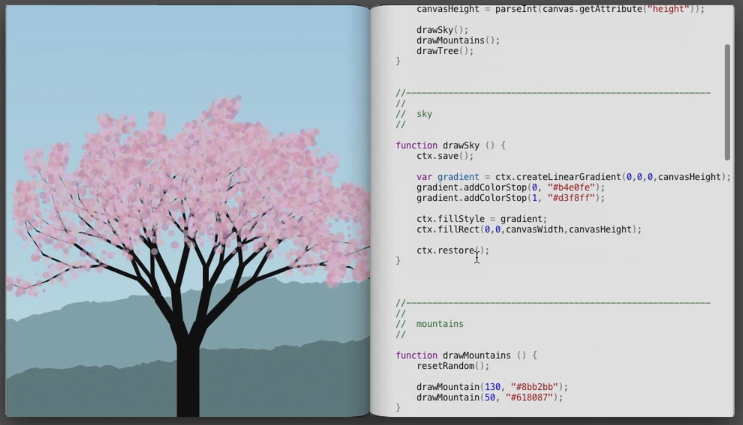
\includegraphics[width=9cm]{fig/bret.png}
  \caption{Live programming: on the right the source code and on the left its instantiation of the code which changes immediately when the code is updated, screenshot from~\cite{Victor2012}.}
  \label{fig:bret}
  \end{center}
\end{figure} 
However, spreadsheets have a number of downsides too. For instance, the lack of  abstraction mechanisms forces spreadsheet users to use copy-paste for reusing code. Although solutions to this problem have been researched~\cite{hermans_2015_19341,jones2003user}, they do not provide the power of full programming languages to spreadsheet users. Secondly, the way formulas are edited in a spreadsheet system like Excel has important drawbacks from the programming perspective. For instance, Excel's formula editor lacks even the basic editor services, such as  syntax highlighting and reference resolution.  In general, the interface is not inviting to apply proper coding styles and practices. Another disadvantage of embedding the code within the sheet itself is that it prohibits versioning and sharing of the formulas separately from the data. 

%\subsection{Code}
On the other hand, there is source code. All existing programming languages support abstraction, and modern editors help developers understand and structure their code. However, mainstream integrated development environments (IDE) lack the live and interactive style of interaction so coveted by spreadsheet users.
% \todo{apart from a few recent initiative that have not been adopted %mainstraim, Tijs, hedd gij dr paraat?} 

%\subsubsection{Directness}
%Another benefit of spreadsheets is that their interface combines data, metadata and calculations together in one view, and provides the user with easy access to all. Just by clicking a formula, one can manipulate it. This is often called `directness': \emph{``the feeling that one is directly manipulating the object''} \cite{shneiderman_direct_1983}. From a cognitive perspective, directness in computing means \emph{``a small distance between a goal and the actions required of the user to achieve the goal''} \cite{burnett_visual_2001}.

%Maloney and Smith describe directness as the fact that a user can \emph{``can initiate the process of examining or changing the attributes, structure, and behavior of user interface components by pointing at their graphical representations directly, as opposed to navigating through an alternate representation.''}\cite{maloney_directness_1995}.

%This almost exactly describes the interface of a spreadsheet. Instead of navigating to a code behind, a class or an object, spreadsheet users have all ingredients: data, metadata and calculations, in one view, and can access them with one click. 
 
In this paper, we will describe \textit{TrueGrid}, a light-weight approach to bridging the gap between programming and spreadsheets and describe ts implications in both worlds. The basic concept of TrueGrid is to allow a spreadsheet like grid to be programmed using a full featured programming language, in a consistent user interface. Figure \ref{fig:TG} shows this idea as implemented in our prototype. 
The key charactertistic is that  developers see the code and data at once. Furthermore, like a spreadsheet, TrueGrid is live, i.e. on a change of data or code, the grid is updated.
In our example, we use JavaScript as a language, however, the idea itself is not limited to a single programming language.
% in fact, one can even image a grid in which different programming languages live.

\begin{figure}
  \begin{center}
  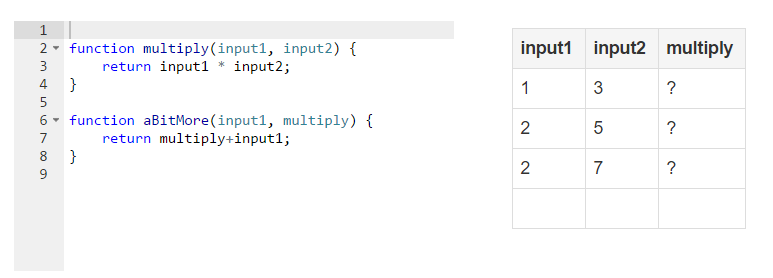
\includegraphics[width=9cm]{fig/TG.png}
  \caption{A True Grid \todo{make ss with syntax highlighting, and add explanation}}
  \label{fig:TG}
  \end{center}
\end{figure} 

In the next section we explore the implication of the TrueGrid user interface for spreadsheet users. Section~\ref{SECT:dev} explores TrueGrid from the perspective of programmers. In particular we discuss conventions for relating code to the grid view. 

\section{TrueGrid for Spreadsheet Users}

As an implementation of TrueGrid for spreadsheet users, we hypothesize that existing spreadsheet system is extended with a source code editor view, next to the grid-based view of the data. This allows users to  use advanced features like PivotTables and charts on top of their TrueGrid, but also use professional IDE services for expressing computations. For spreadsheet users, using TrueGrid over spreadsheets presents several benefits. For example, the use of a professional  editor supports the developer with editor services like syntax highlighting and error marking. Furthermore, the textual form of the code allows for easy diffing and merging, enabling more mature version control on spreadsheets. While learning a new programming language can be challenging, there are spreadsheet developers working with VBA now, which is a fully featured language. Unfortunately the integration between the code and a spreadsheet is low level and cumbersome. We envision TrueGrid having a lower lower learning curve because code and data are juxtaposed.

\begin{figure}[t]
\begin{minipage}{0.6\linewidth}
\begin{lstlisting}
function column_avg(row) {
  return (row.lab + row.exam) / 2;
}

function cell_classAvg(col, row) {   
  return sum(col) / col.length; 
}
\end{lstlisting}
\end{minipage}
\begin{minipage}{0.38\linewidth}
\centering
\sffamily
\begin{tabular}{|c|c|c|c|}\hline
student & lab & exam & avg\\\hline\hline
Rich   & 7 & 8 & 7.5 \\\hline
Jacome & 8 & 9 & 8.5\\\hline
Birgit & 9 & 9 & 9 \\\hline
 & & & \textit{classAvg:} 8.3 \\\hline
\end{tabular}
\end{minipage}
\caption{Mockup of TrueGrid for spreadsheet use}
\label{FIG:grades}
\end{figure}

As an example consider the simple grade book sheet shown in Fig.~\ref{FIG:grades}. It shows the actual data (both provided and computed) in the grid. The average and class average are expressed using ordinary Javascript functions. The TrueGrid environment links functions or methods to the cells in the grid using a naming convention.
For instance, function starting with the \lstinline{column_} prefix computes a complete column, given a particular row (an ordinary Javascript object).
This is used in the computation of the \lstinline{avg} column, where each cell contains the average of the lab and exam cells.
The model also allows naming individual cells. This is illustrated in the function \lstinline{cell_classAvg}. The function receives the current column (\lstinline{col}, a Javascript array), and the current \lstinline{row}. Based on the elements in the column the class average is computed. 

One could imagine linking the code to the grid using row and column coordinates, just like ordinary spreadsheet formulas refer to (ranges of) rows and columns. However, this would lead to code that is not very intuitive if read separately. Furthermore,  insertion of rows and columns in the grid would require updating the source code itself, similar to how spreadsheet systems realign cell coordinates. 


\section{TrueGrid for Developers}
\label{SECT:dev} 

%In this section we switch perspective, and explore how TrueGrid can be beneficial for  professional programmers as well. 
Like spreadsheet users, developers often work with (example) data when programming. For instance, developers use read-eval-print-loops (REPLs) to explore the behavior of a function. 
Another use case is developer testing which requires setting up test fixtures and inspecting the results.
Both these use cases, however, suffer from a lack of immediacy. After a change to the code, the developer needs to reenter expressions in the REPL to observe expected changes in behavior. Similar for testing: reexecuting the test is an explicit step after every change to the code. TrueGrid  eliminates these hickups and promises a more fluent, live experience. 

\begin{figure}[t]
\begin{minipage}{0.6\linewidth}
\begin{lstlisting}
function leftpad(str, len, ch) {
  str = String(str);
  var i = -1;
  if (!ch && ch !== 0) ch = ' ';
  len = len - str.length;
  while (++i < len) {
    str = ch + str;
  }
  return str;
}
\end{lstlisting}
\end{minipage}
\begin{minipage}{0.4\linewidth}
\centering
\sffamily
\begin{tabular}{|c|c|m{0.5cm}|p{0.5cm}|c|}\hline
function & 0 & 1 & 2 & Result \\\hline\hline
leftpad & "foo" & 5 &  & "  foo" \\\hline
leftpad & "foobar" & 6 & & "foobar" \\\hline
leftpad & 1 & 2 & 0 & "01"\\\hline
\end{tabular}
\end{minipage}
\caption{Exploring function behavior using TrueGrid}
\label{FIG:leftpad}
\end{figure}

In particular, TrueGrid can be seen as a persistent REPL, where expressions or method invocations are continuously evaluated, after every change to the code or input data. 
Consider the example shown in Fig.~\ref{FIG:leftpad}.
On the left is a simple Javascript function for left-padding values with spaces or other padding characters. 
Using TrueGrid, the programmer can provide example data in the grid and explore the implementation. This can be especially valuable early in the development process when  you have some data and only a vague idea of where the how certain functionality should be implemented.

From the testing perspective, TrueGrid provides a kind of ``FIT testing on steroids''~\cite{mugridge2005fit}, where the grid functions as a live dashboard of test success and failure. 
In this case, the grid shown in Fig.~\ref{FIG:leftpad} could have an additional column indicating the success or failure of the function execution, or use green/red coloring of rows to the same effect.
Again, the success indicators would be automatically updated upon changing the source code on left. 


\section{Conclusion and Outlook}

Spreadsheets are live programming environments. However, their lack of abstraction mechanisms and editor support are impediments to professional spreadsheet development. Conversely, traditional programming environments lack the continuos feedback that make spreadsheets so attractive. In this paper we have presented TrueGrid, a user interface design combining code editing and grid-based data view, with a live execution model.

TrueGrid presents a promising bridge between the domain of spreadsheets and software development. It has the potential to improve end-user programming experience from two perspectives:
\begin{itemize}
\item For spreadsheet users: computations are expressed using program code, instead of  formulas in cells, so that end-users may enjoy both abstraction and liveness at the same time.
\item For professional developers: spreadsheet-like grids support live exploration and testing of code, without explicitly invoking test scripts of entering expressions in a REPL.
\end{itemize}
We have implemented a prototype of TrueGrid which runs in the browser, using Javascript as the programming language. Further research is needed to empirically investigate the benefits of TrueGrid from both the programmer and spreadsheet user perspectives. 
We expect that TrueGrid provides a fruitful vehicle for exploring the middle ground between full end-user programming, and professional software development. 


\bibliographystyle{splncs03}
\bibliography{references}
\end{document}